% This file is part of template-latex-project.
%
% template-latex-project is free software: you can redistribute it and/or modify
% it under the terms of the GNU General Public License as published by
% the Free Software Foundation, either version 3 of the License, or
% (at your option) any later version.
%
% template-latex-project is distributed in the hope that it will be useful,
% but WITHOUT ANY WARRANTY; without even the implied warranty of
% MERCHANTABILITY or FITNESS FOR A PARTICULAR PURPOSE.  See the
% GNU General Public License for more details.
%
% You should have received a copy of the GNU General Public License
% along with template-latex-project. If not, see <https://www.gnu.org/licenses/>.

\documentclass[aps,prl,twocolumn,groupedaddress]{revtex4-2}

% ---------------------------------------------------------------------------------------------------------------------
% Packages
% ---------------------------------------------------------------------------------------------------------------------

\usepackage{amsmath}
\usepackage{amsfonts}
\usepackage{amssymb}
\usepackage{bm}
\usepackage{comment}
\usepackage{enumitem}
\usepackage{geometry}
\usepackage{graphicx}
\usepackage{hyperref}
\usepackage[utf8]{inputenc}
\usepackage{layout}
\usepackage{textcomp}
\usepackage{ulem}
\usepackage{xcolor}

% ---------------------------------------------------------------------------------------------------------------------
% Preamble
% ---------------------------------------------------------------------------------------------------------------------

% This file is part of template-latex-project.
%
% template-latex-project is free software: you can redistribute it and/or modify
% it under the terms of the GNU General Public License as published by
% the Free Software Foundation, either version 3 of the License, or
% (at your option) any later version.
%
% template-latex-project is distributed in the hope that it will be useful,
% but WITHOUT ANY WARRANTY; without even the implied warranty of
% MERCHANTABILITY or FITNESS FOR A PARTICULAR PURPOSE.   See the
% GNU General Public License for more details.
%
% You should have received a copy of the GNU General Public License
% along with template-latex-project. If not, see <https://www.gnu.org/licenses/>.

% ---------------------------------------------------------------------------------------------------------------------
% geometry
% ---------------------------------------------------------------------------------------------------------------------

\geometry{
	a4paper,
	total={170mm,257mm},
	left=20mm,
	top=20mm,
}

% ---------------------------------------------------------------------------------------------------------------------
% graphicx
% ---------------------------------------------------------------------------------------------------------------------

\graphicspath{
	{./content/figures}
}

% ---------------------------------------------------------------------------------------------------------------------
% hyperref
% ---------------------------------------------------------------------------------------------------------------------

\hypersetup{
	colorlinks=true,
	urlcolor=black,
	citecolor=black,
	linkcolor=black,
}


% ---------------------------------------------------------------------------------------------------------------------
% Body
% ---------------------------------------------------------------------------------------------------------------------

\begin{document}

\title{Example Paper}

\author{Egon E. Braun Filho}
\email[]{egon@mundoalem.io}
\homepage[]{https://www.mundoalem.io/}
\thanks{My family.}
\affiliation{Mundoalem}

\date{\today}

\begin{abstract}
	This in an example paper written in \LaTeX{} and following the conventions set by \emph{revtex}. Source files are
	available in the following git repository: \url{https://github.com/mundoalem/template-latex-project}.
\end{abstract}

\maketitle

% This file is part of template-latex-project.
%
% template-latex-project is free software: you can redistribute it and/or modify
% it under the terms of the GNU General Public License as published by
% the Free Software Foundation, either version 3 of the License, or
% (at your option) any later version.
%
% template-latex-project is distributed in the hope that it will be useful,
% but WITHOUT ANY WARRANTY; without even the implied warranty of
% MERCHANTABILITY or FITNESS FOR A PARTICULAR PURPOSE.  See the
% GNU General Public License for more details.
%
% You should have received a copy of the GNU General Public License
% along with template-latex-project. If not, see <https://www.gnu.org/licenses/>.

% This file is part of template-latex-project.
%
% template-latex-project is free software: you can redistribute it and/or modify
% it under the terms of the GNU General Public License as published by
% the Free Software Foundation, either version 3 of the License, or
% (at your option) any later version.
%
% template-latex-project is distributed in the hope that it will be useful,
% but WITHOUT ANY WARRANTY; without even the implied warranty of
% MERCHANTABILITY or FITNESS FOR A PARTICULAR PURPOSE.  See the
% GNU General Public License for more details.
%
% You should have received a copy of the GNU General Public License
% along with template-latex-project. If not, see <https://www.gnu.org/licenses/>.

\section{\label{sec:Introduction}Introduction}

Lorem ipsum dolor sit amet, consectetur adipiscing elit. Quisque et diam aliquam, feugiat sem eget, condimentum dui.
Etiam metus justo, aliquam nec enim et, dictum fermentum augue. Duis justo massa, fermentum nec malesuada eget, gravida
et libero. Praesent laoreet accumsan finibus. Donec diam tortor, congue eget euismod in, facilisis nec mauris. Donec
eleifend, augue aliquet tincidunt auctor, nibh sem elementum erat, sit amet sagittis ante ipsum eget sapien. Donec diam
ligula, commodo porttitor eleifend a, fermentum eu sapien. Proin lacus quam, interdum in tempus a, consequat non
libero. Phasellus tristique bibendum justo.

Pellentesque nec efficitur diam. Donec a dictum tellus, quis vehicula diam. Maecenas ultrices id diam sit amet
elementum. Curabitur tincidunt consectetur arcu et luctus. Nullam gravida, metus id consectetur lacinia, eros diam
maximus tortor, ac scelerisque orci lectus a lacus. Nulla in luctus turpis. Donec feugiat vitae elit vitae aliquam.
Curabitur lacinia imperdiet rutrum. Fusce et sagittis mi, id vehicula risus. Aenean quis nisl sapien. Proin vel quam
viverra, consectetur mauris et, rutrum turpis. Cras in imperdiet dolor.

% This file is part of template-latex-project.
%
% template-latex-project is free software: you can redistribute it and/or modify
% it under the terms of the GNU General Public License as published by
% the Free Software Foundation, either version 3 of the License, or
% (at your option) any later version.
%
% template-latex-project is distributed in the hope that it will be useful,
% but WITHOUT ANY WARRANTY; without even the implied warranty of
% MERCHANTABILITY or FITNESS FOR A PARTICULAR PURPOSE.  See the
% GNU General Public License for more details.
%
% You should have received a copy of the GNU General Public License
% along with template-latex-project. If not, see <https://www.gnu.org/licenses/>.

\section{\label{sec:usinglists}Using Lists Example}

Lorem ipsum dolor sit amet, consectetur adipiscing elit. Quisque et diam aliquam, feugiat sem eget, condimentum dui.
Etiam metus justo, aliquam nec enim et, dictum fermentum augue. Duis justo massa, fermentum nec malesuada eget, gravida
et libero. Praesent laoreet accumsan finibus.

\begin{enumerate}
	\item Lorem ipsum dolor sit amet.
	\item Consectetur adipiscing elit.
	\item Quisque et diam aliquam, feugiat sem eget, condimentum dui.
	\item Etiam metus justo:
	      \begin{itemize}
		      \item Subitem 1
		      \item Subitem 2
		      \item Subitem 3
	      \end{itemize}
	\item Praesent laoreet accumsan finibus.
\end{enumerate}

Nulla in luctus turpis. Donec feugiat vitae elit vitae aliquam. Curabitur lacinia imperdiet rutrum. Fusce et sagittis
mi, id vehicula risus.


% This file is part of template-latex-project.
%
% template-latex-project is free software: you can redistribute it and/or modify
% it under the terms of the GNU General Public License as published by
% the Free Software Foundation, either version 3 of the License, or
% (at your option) any later version.
%
% template-latex-project is distributed in the hope that it will be useful,
% but WITHOUT ANY WARRANTY; without even the implied warranty of
% MERCHANTABILITY or FITNESS FOR A PARTICULAR PURPOSE.  See the
% GNU General Public License for more details.
%
% You should have received a copy of the GNU General Public License
% along with template-latex-project. If not, see <https://www.gnu.org/licenses/>.

\section{\label{sec:usingmath}Using Math Example}

Lorem ipsum dolor sit amet, consectetur adipiscing elit. Quisque et diam aliquam, feugiat sem eget, condimentum dui.
Etiam metus justo, aliquam nec enim et, dictum fermentum augue. Duis justo massa, fermentum nec malesuada eget, gravida
et libero. Praesent laoreet accumsan finibus. Nulla in luctus turpis. Donec feugiat vitae elit vitae aliquam. Curabitur
lacinia imperdiet rutrum. Fusce et sagittis mi, id vehicula risus.

\begin{equation}
	a^2+b^2=c^2 \,.
	\label{eqn:pythagoras}
\end{equation}

Lorem ipsum dolor sit amet, consectetur adipiscing elit. Quisque et diam aliquam, feugiat sem eget, condimentum dui.
Etiam metus justo, aliquam nec enim et, dictum fermentum augue. Duis justo massa, fermentum nec malesuada eget, gravida
et libero. Praesent laoreet accumsan finibus. Nulla in luctus turpis. Donec feugiat vitae elit vitae aliquam. Curabitur
lacinia imperdiet rutrum. Fusce et sagittis mi, id vehicula risus.

% This file is part of template-latex-project.
%
% template-latex-project is free software: you can redistribute it and/or modify
% it under the terms of the GNU General Public License as published by
% the Free Software Foundation, either version 3 of the License, or
% (at your option) any later version.
%
% template-latex-project is distributed in the hope that it will be useful,
% but WITHOUT ANY WARRANTY; without even the implied warranty of
% MERCHANTABILITY or FITNESS FOR A PARTICULAR PURPOSE.  See the
% GNU General Public License for more details.
%
% You should have received a copy of the GNU General Public License
% along with template-latex-project. If not, see <https://www.gnu.org/licenses/>.

\section{\label{sec:usingtables}Using Tables Example}

Quisque et diam aliquam, feugiat sem eget, condimentum dui. Etiam metus justo, aliquam nec enim et, dictum fermentum
augue. Duis justo massa, fermentum nec malesuada eget, gravida et libero. Praesent laoreet accumsan finibus. Nulla in
luctus turpis. Donec feugiat vitae elit vitae aliquam. Curabitur lacinia imperdiet rutrum. Fusce et sagittis mi, id
vehicula risus.

\begin{table}[h!]\label{tab:tableexample}
	\begin{center}
		\caption{Example.}
		\begin{tabular}{l|c|c}
			\hline
			Header 1 & Header 2 & Header 3 \\
			\hline \hline
			Value 1  & Value 2  & Value 3  \\
			Value 1  & Value 2  & Value 3  \\
			Value 1  & Value 2  & Value 3  \\
			Value 1  & Value 2  & Value 3  \\
			Value 1  & Value 2  & Value 3  \\
			\hline
		\end{tabular}
	\end{center}
\end{table}

Duis justo massa, fermentum nec malesuada eget, gravida et libero. Praesent laoreet accumsan finibus. Nulla in luctus
turpis. Donec feugiat vitae elit vitae aliquam. Curabitur lacinia imperdiet rutrum. Fusce et sagittis mi, id vehicula
risus.

% This file is part of template-latex-project.
%
% template-latex-project is free software: you can redistribute it and/or modify
% it under the terms of the GNU General Public License as published by
% the Free Software Foundation, either version 3 of the License, or
% (at your option) any later version.
%
% template-latex-project is distributed in the hope that it will be useful,
% but WITHOUT ANY WARRANTY; without even the implied warranty of
% MERCHANTABILITY or FITNESS FOR A PARTICULAR PURPOSE.  See the
% GNU General Public License for more details.
%
% You should have received a copy of the GNU General Public License
% along with template-latex-project. If not, see <https://www.gnu.org/licenses/>.

\section{\label{sec:usingfigures}Using Figures Example}

Lorem ipsum dolor sit amet, consectetur adipiscing elit. Quisque et diam aliquam, feugiat sem eget, condimentum dui.
Etiam metus justo, aliquam nec enim et, dictum fermentum augue. Duis justo massa, fermentum nec malesuada eget, gravida
et libero. Praesent laoreet accumsan finibus. Nulla in luctus turpis.

\begin{figure}[h]\label{fig:example}
	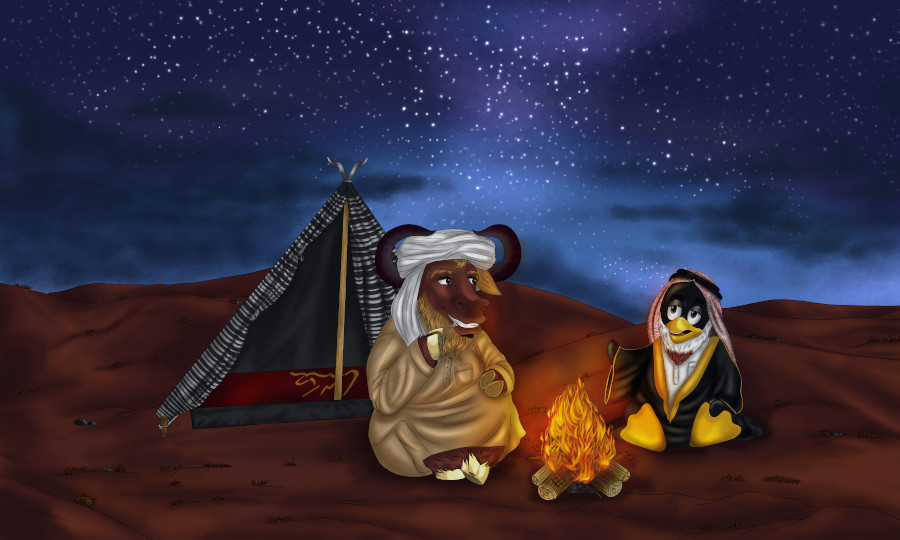
\includegraphics[clip=true, width=\columnwidth]{example}
	\caption{Gnu and Tux Bivouac}
\end{figure}

Duis justo massa, fermentum nec malesuada eget, gravida et libero. Praesent laoreet accumsan finibus. Nulla in luctus
turpis. Donec feugiat vitae elit vitae aliquam. Curabitur lacinia imperdiet rutrum.

% This file is part of template-latex-project.
%
% template-latex-project is free software: you can redistribute it and/or modify
% it under the terms of the GNU General Public License as published by
% the Free Software Foundation, either version 3 of the License, or
% (at your option) any later version.
%
% template-latex-project is distributed in the hope that it will be useful,
% but WITHOUT ANY WARRANTY; without even the implied warranty of
% MERCHANTABILITY or FITNESS FOR A PARTICULAR PURPOSE.  See the
% GNU General Public License for more details.
%
% You should have received a copy of the GNU General Public License
% along with template-latex-project. If not, see <https://www.gnu.org/licenses/>.

\section{\label{sec:usingcitations}Using Citations Example}

Lorem ipsum dolor sit amet, consectetur adipiscing elit. Lorem~\cite{ExampleArticle}, feugiat sem eget, condimentum dui.
Justo, aliquam nec enim et, dictum augue. Duis~\cite{ExampleBook} justo massa, fermentum nec malesuada eget. Curabitur
praesent laoreet accumsan finibus. Nulla in luctus turpis. Donec feugiat vitae elit vitae aliquam. Curabitur lacinia
imperdiet rutrum. Fusce et sagittis mi, id vehicula risus.

Lorem ipsum dolor sit amet, consectetur adipiscing elit. Lorem~\cite{ExampleUrl}, feugiat sem eget, condimentum dui. Et
praesent laoreet accumsan finibus. Nulla in luctus turpis. Donec feugiat vitae elit vitae aliquam. Curabitur lacinia
imperdiet rutrum. Fusce et sagittis mi, id vehicula risus.



% This file is part of template-latex-project.
%
% template-latex-project is free software: you can redistribute it and/or modify
% it under the terms of the GNU General Public License as published by
% the Free Software Foundation, either version 3 of the License, or
% (at your option) any later version.
%
% template-latex-project is distributed in the hope that it will be useful,
% but WITHOUT ANY WARRANTY; without even the implied warranty of
% MERCHANTABILITY or FITNESS FOR A PARTICULAR PURPOSE.  See the
% GNU General Public License for more details.
%
% You should have received a copy of the GNU General Public License
% along with template-latex-project. If not, see <https://www.gnu.org/licenses/>.

\appendix
% This file is part of template-latex-project.
%
% template-latex-project is free software: you can redistribute it and/or modify
% it under the terms of the GNU General Public License as published by
% the Free Software Foundation, either version 3 of the License, or
% (at your option) any later version.
%
% template-latex-project is distributed in the hope that it will be useful,
% but WITHOUT ANY WARRANTY; without even the implied warranty of
% MERCHANTABILITY or FITNESS FOR A PARTICULAR PURPOSE.  See the
% GNU General Public License for more details.
%
% You should have received a copy of the GNU General Public License
% along with template-latex-project. If not, see <https://www.gnu.org/licenses/>.

\section{\label{sec:appendixa}Appendix A}

Lorem ipsum dolor sit amet, consectetur adipiscing elit. Quisque et diam aliquam, feugiat sem eget, condimentum dui.
Etiam metus justo, aliquam nec enim et, dictum fermentum augue. Duis justo massa, fermentum nec malesuada eget, gravida
et libero. Praesent laoreet accumsan finibus. Donec diam tortor, congue eget euismod in, facilisis nec mauris. Donec
eleifend, augue aliquet tincidunt auctor, nibh sem elementum erat, sit amet sagittis ante ipsum eget sapien. Donec diam
ligula, commodo porttitor eleifend a, fermentum eu sapien. Proin lacus quam, interdum in tempus a, consequat non
libero. Phasellus tristique bibendum justo.

Pellentesque nec efficitur diam. Donec a dictum tellus, quis vehicula diam. Maecenas ultrices id diam sit amet
elementum. Curabitur tincidunt consectetur arcu et luctus. Nullam gravida, metus id consectetur lacinia, eros diam
maximus tortor, ac scelerisque orci lectus a lacus. Nulla in luctus turpis. Donec feugiat vitae elit vitae aliquam.
Curabitur lacinia imperdiet rutrum. Fusce et sagittis mi, id vehicula risus. Aenean quis nisl sapien. Proin vel quam
viverra, consectetur mauris et, rutrum turpis. Cras in imperdiet dolor.



\bibliography{content/references}

\end{document}
